\section{研究内容}\label{sec2}
研究についての具体的な内容を2節以降で記述する.
各節のタイトルは任意.ただし結論,今後の課題,謝辞,参考文献など,論文
としての常識的な項目は必ず入れなければならない.詳しくは卒業研究
担当教員の指導に従うこと.


\subsection{図,表のキャプションと参照}

図や表には必ず題名と参照番号を記述すること.参照番号はlabel を使って自
動的に作成するようにし,ref を使って本文中で参照できるようにしておく.

\begin{figure}[htbp]
  \begin{center}
     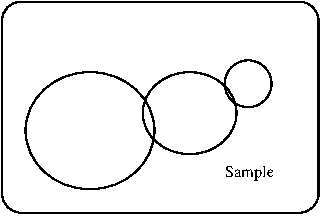
\includegraphics[width=13cm,height=12cm,keepaspectratio]{figure.pdf}\\
     %includegraphicsの詳しい使い方ははLaTeXの参考書を参照.
  \end{center}
  \caption{図の例}%
\label{fig1}
\end{figure}

図や表を入れた場合,必ず図の参照番号を使った文章が本文中にあるはずである.例えば
次のようにすればよい.図\ref{fig1} は図のサンプルである.\TeX のソース
を見ると図の入れ方がわかる.

図が単独で現れ,本文中に何の説明もなければ,ただのページ稼ぎと見なされ
る.

\subsection{参考文献の引用}
参考文献は,本研究が十分な調査活動を基礎として成り立っていることを
明示する,大変重要な項目である.
研究で参考とした文献のリストを論文の終わりに入れ,
それらの文献に関係のある記述部分や,文献に書いてある文章の引用を本文内で行なって
ある箇所には必ず参考文献の番号を入れなければならない.例えば次のよう
にすれば良い.本手引きや予稿の手引きを作成する際,文献
\cite{kinosita}を参考にした.また\LaTeX の各種コマンドに関する説
明は文献\cite{okumura}を参考にした.\TeX \cite{knuth} とは,Knuth によっ
て作られた組版用のソフトウェアのことである.文献\cite{labelName}は,論
文を参照する場合のサンプルである.



本手引き書ではbibitem を用いて直接参考文献リストを本文末尾に記入してい
るが,出来れば文献データベースから参考文献リストを自動的に作成する
\BibTeX 等を使用した方が良い.本手引書の\LaTeX ソースと共に,\BibTeX の
データベースファイルも配布する.\BibTeX の詳しい使用方法については,
文献\cite{okumura}等\LaTeX の参考書を参照のこと.

\subsection{各節の引用}
各節にも label をつけておいて,後の節で節番号を使って自動的に引用番号
を記述できるようにしておくと良いだろう.例えば次のようにすれば良い.
\ref{sec1}節で述べた目的を達成するため,本節では次のような方法を用いた
場合につい述べる.$\cdots$

label とref を用いた参照は 図のキャプションや section, subsection だけ
でなく,数式等にも使えるので,番号を手でつけることは出来るだけ控え,
自動的な番号づけと参照を行ない間違いのない文章になるようにしよう.